\documentclass[12pt,a4paper]{report}
\usepackage[utf8]{vietnam}\usepackage{amsmath, amsthm, amssymb,latexsym,amscd,amsfonts,enumerate}
\usepackage[top=2.5cm, bottom=2.3cm, left=2.3cm, right=2.5cm]{geometry} 
\usepackage{color, fancyhdr, graphicx, wrapfig}
\usepackage[unicode]{hyperref}
\usepackage[vietnamese]{babel}
\usepackage{amsthm}
\usepackage{amsmath}
\usepackage{amsfonts}	
\usepackage{mathtools}
\usepackage{ulem}
\usepackage{longtable}
\usepackage{float}
\usepackage{amssymb}
\usepackage{tkz-euclide}
\usepackage{tikz,tkz-tab}
\usepackage{empheq} %gói móc nhọn cho hệ pt
\usepackage{graphicx} 
\usepackage{hhline} % Sử dụng gói lệnh hhline
\usepackage{ltablex}% gói tách bảng khi quá dài
\usepackage{titling}
\usepackage{nicematrix}
\usepackage{secdot}
\usepackage{enumitem}
\usepackage{enumerate}
\usepackage{array}
\usepackage{multirow}
\usetikzlibrary{calc}
\usepackage{longtable}
\usepackage{indentfirst}
\usepackage{fancyhdr}
\usepackage[bottom]{footmisc}

\usepackage{tocloft}
\usepackage{xcolor}
\usepackage{listings}
\renewcommand{\cftchapfont}{\color{red!85}}       % Chương

\usepackage[labelfont=bf]{caption}
\everymath{\displaystyle}

\usepackage{exscale,relsize,makeidx}
%\usepackage{refcheck}

\definecolor{babyblue}{rgb}{0.54, 0.81, 0.94}
\definecolor{blizzardblue}{rgb}{0.67, 0.9, 0.93}

\setcounter{tocdepth}{4}
\setcounter{secnumdepth}{4}
\numberwithin{equation}{section}
\theoremstyle{definition} %định nghĩa chữ thường không in nghiêng cho các môi trường định nghĩa toán học
\newtheorem{dn}{Định nghĩa}[chapter]
\newtheorem{tc}{Tính chất}[chapter]
\newtheorem{dl}{Định lý}[chapter]
\newtheorem{md}{Mệnh đề}[chapter]
\newtheorem{bd}{Bổ đề}[chapter]
\newtheorem{hq}{Hệ quả}[chapter]
\newtheorem{nx}{Nhận xét}[chapter]
\newtheorem{vd}{Ví dụ}[chapter]
\newtheorem{cy}{Chú ý}[chapter]
\pagenumbering{roman}\pagestyle{plain}
%\pagestyle{fancy}chapter
%\lhead{\it \changefontsizes{11pt}Luận văn thạc sĩ:}
%\rhead{\it Một số phương pháp vô hướng hóa cơ bản trong tối ưu đa mục tiêu}
%\lfoot{\it Nguyễn Văn Vân } 			         
%\rfoot{\it K19.2 trường ĐHSG}
\renewcommand{\headrulewidth}{1,2pt} 	
\renewcommand{\arraystretch}{1.3}%tạo dọ cao cho dòng		


\newcommand{\dstc}[2]
{
	\newdimen\stringwidth\setbox0=\hbox{#1}
	\stringwidth=\wd0
	\hspace*{-\parindent}\hspace*{.5\textwidth}\hspace*{-.5\wd0}#1\hfill #2\bigskip
}  
\lstset{
    language=Python,
    basicstyle=\ttfamily\small,
    keywordstyle=\color{blue},
    stringstyle=\color{red!70!brown},
    commentstyle=\color{green!50!black},
    numbers=left,
    numberstyle=\tiny,
    breaklines=true,
    showstringspaces=false,
    frame=single
}
\usepackage{scrextend}
\fancyhf{}
\lhead{}
\chead{\thepage}
\rhead{}
\cfoot{}
\rfoot{}
\lfoot{}
\pagestyle{fancy}
\renewcommand{\headrulewidth}{0.5pt}

%\changefontsizes{13pt}

\begin{document} 
	\begin{titlepage}
	\begin{tikzpicture}[remember picture, overlay]
		
		\draw[line width = 1.5pt] ($(current page.north west) + (1in,-0.8in)$) rectangle ($(current page.south east) + (-0.6in,0.8in)$);
		
	\end{tikzpicture}
	\centering
	\textbf{ỦY BAN NHÂN DÂN THÀNH PHỐ HỒ CHÍ MINH\smallskip\\
		TRƯỜNG ĐẠI HỌC SÀI GÒN}\par
	\rule{5cm}{0.5pt}\par
	
	
	
	\begin{figure}[h]
		\centering
		
\includegraphics[width=6cm]{img/logodhsg.png}
		
	\end{figure}
	
	\vspace{1cm}
	{\Huge\textbf{BÁO CÁO TỔNG KẾT \\ \hspace{0.5cm} ĐỒ ÁN MÔN HỌC\\PHÂN TÍCH VÀ XỬ LÝ ẢNH}\par}
	\vspace{3cm}
	{\Huge\textbf{Xử lý ảnh trên miền tần số \\(Image Enhancement in the Frequency Domain) }\par}
	% \large\textbf{ Thuộc nhóm ngành khoa học: Toán-Ứng dụng\\ Chủ nhiệm đề tài: Nguyễn Thành Nam }\par		
	\vspace{2cm}
	\large{\textbf{Giảng viên hướng dẫn: PGS.TS Phạm Thế Bảo}}
	\vfill
	\textbf{Thành phố Hồ Chí Minh, tháng 11  năm 2025}
\end{titlepage}



\begin{titlingpage} %BÌA PHỤ II
	\begin{tikzpicture}[remember picture, overlay]
		\draw[line width = 1.5pt] ($(current page.north west) + (1in,-0.8in)$) rectangle ($(current page.south east) + (-0.6in,0.8in)$);
		
	\end{tikzpicture}
	\centering
	\textbf{ỦY BAN NHÂN DÂN THÀNH PHỐ HỒ CHÍ MINH\smallskip\\
		TRƯỜNG ĐẠI HỌC SÀI GÒN}\par
	\rule{5cm}{0.5pt}\par
	\vspace{5cm}
	
	
	\vspace{1cm}
	{\Large\textbf{BÁO CÁO TỔNG KẾT \\ \hspace{0.5cm} ĐỒ ÁN MÔN HỌC \\
  PHÂN TÍCH VÀ XỬ LÝ ẢNH}\par}
	\vspace{2cm}
	{\Large\textbf{Xử lý ảnh trên miền tần số \\(Image Enhancement in the Frequency Domain)}\par}
	\vspace{3cm}
	
	\large\textbf{ }\par		
	
	\large{}
	\vspace{1.5cm}
	
\begin{tabular}{|c|c|}
  \hline
  MSV & Họ và tên  \\ 
	\hline
	   3122480001  &   Trần Đức Anh                    \\
  \hline
   3122480034  &  Nguyễn Thành Nam                       \\ 
  \hline
   3122480042  &   Bùi Tấn Phát                       \\ 
  \hline
 \end{tabular}

	\vspace{0.8cm}
	
	
	
	%	\includegraphics[height=2cm]{chukynew}
	\vfill
	\textbf{Thành phố Hồ Chí Minh, tháng 11  năm 2025}
\end{titlingpage}
	
	%\large
	\renewcommand{\baselinestretch}{1.2}
	\fontsize{13pt}{20pt}\selectfont
	
	\chapter*{Lời cam đoan}
	\thispagestyle{fancy}
	\addcontentsline{toc}{chapter}{Lời cam đoan}
	\vspace{1cm}
	\indent
	
	Tôi tên là Nguyễn Thành Nam, Sinh viên lớp DTU1221, Khoa Toán-Ứng dụng, Khóa 22,  thuộc trường Đại học Sài Gòn.
	
	 Tôi xin cam đoan toàn bộ nội dung được trình bày trong bản báo cáo này  đều do chính tôi thực hiện dưới sự hướng dẫn của \textit{PGS.TS Phạm Thế Bảo}. Những kết quả nghiên cứu của tác giả khác được sử dụng trong đề tài  đều có trích dẫn đầy đủ. Tôi xin hoàn toàn chịu trách nhiệm nếu có các nội dung sao chép không hợp lệ hoặc vi phạm quy chế đào tạo. 
	\\
	\\
	\\
	\rightline{{\it {Tp. HCM, tháng 11  năm 2025}} \hspace*{0cm}}
	\rightline{\textbf{Tác giả} \hspace*{2cm}}

	
	%\vspace*{1cm}
	\rightline{\textbf{Nguyễn Thành Nam}\hspace*{0.9cm}}
	
	\chapter*{Lời cảm ơn}
	\thispagestyle{fancy}
	\addcontentsline{toc}{chapter}{Lời cảm ơn}
	\vspace{1cm}
	\indent
	
Tiểu luận này được hoàn thành tại trường Đại Học Sài Gòn dưới sự hướng dẫn của \textit{PGS.TS Phạm Thế Bảo}. Em xin bày tỏ lòng biết ơn chân thành và sâu sắc về sự tận tâm và nhiệt tình của Thầy trong suốt quá trình tác giả thực hiện đề tài.
	
	
	\bigskip
	Xin cám ơn Phòng Đào tạo  và Khoa Toán - Ứng dụng trường Đại học Sài Gòn, gia đình, bạn bè  và các thầy cô đã tạo nhiều điều kiện thuận lợi, giúp em hoàn thành đồ án môn học này.
	\\
	\\
	\\
	\rightline{{\it {Tp. HCM, tháng 11  năm 2025}} \hspace*{0cm}}
	\rightline{\textbf{ Tác giả} \hspace*{2cm}}

	
	%\vspace*{1cm}
	\rightline{\textbf{Nguyễn Thành Nam}\hspace*{0.9cm}}
	\newpage
	
	\addcontentsline{toc}{chapter}{Mục lục}
	\tableofcontents
	%\thispagestyle{plain}

	\chapter*{Danh mục các từ viết tắt  }
\thispagestyle{fancy}
\addcontentsline{toc}{chapter}{Danh mục các từ viết tắt}
\vspace{1cm}
\indent

\begin{center}
	\begin{tabular}{ |p{3cm}|p{5cm}|  }
		\hline
		DFT & Discrete Fourier Transforms  \\ \hline
		IDFT & Inverse Discrete Fourier Transforms  \\ \hline
		 & Phương án tối ưu \\ \hline
			 & Phương án\\ \hline
		& Bài toán  \\ \hline
	
		\hline
	\end{tabular}
\end{center}

	\chapter*{Danh mục các bảng, hình vẽ  }
\thispagestyle{fancy}
\addcontentsline{toc}{chapter}{Danh mục các bảng, hình vẽ}
\vspace{1cm}
\indent

\begin{longtable}{l   l }
	\textbf{Hình, bảng}  & \textbf{Trang}       \\
	%Hình \ref{hinhdothi} Nghiệm tối ưu của BT \ref{1133}. &       \pageref{hinhdothi}       \\
	%Hình \ref{hinhthamso1}  Ví dụ \ref{2211}- BT có hàm mục tiêu không bị chặn. &       \pageref{hinhthamso1}         \\
	%Hình \ref{hinhthamso2} Ví dụ \ref{2211}- BT đạt tối ưu.  &      \pageref{hinhthamso2}     \\
	%Hình \ref{hinhthamso3} Ví dụ \ref{2211}- BT vẫn đạt tối ưu. &       \pageref{hinhthamso3}     \\
	%Bảng đơn hình \ref{1-0} - \ref{3-0} Ví dụ \ref{122} - BT chứa tham số ở vế phải.  &   \pageref{1-0} \\
	%Bảng đơn hình \ref{4-0} - \ref{5-0} Ví dụ \ref{2222} - TH2 BT chứa tham số ở hàm mục tiêu. &   \pageref{4-0} \\
	%Bảng đơn hình \ref{6-0} - \ref{10-0} Ví dụ \ref{2233} - TH3 BT chứa tham số ở hàm mục tiêu. &   \pageref{6-0} \\
	%Bảng đơn hình \ref{11-0} - \ref{13-0} Ví dụ \ref{2244} - BT chứa tham số ở hàm mục tiêu. &   \pageref{11-0} \\
 %từ 14-0 là chương 3
 %Bảng đơn hình \ref{14-0} - \ref{20-0} Ví dụ \ref{3322} - BT phân thức chứa tham số hàm mục tiêu. &   \pageref{14-0} \\


\end{longtable}


	\newpage
	\pagenumbering{arabic} 
	\chapter*{Lời nói đầu}
	\thispagestyle{fancy}
	\addcontentsline{toc}{chapter}{{\bf  Lời nói đầu}\rm}
	\renewcommand{\baselinestretch}{1.2}

	
\vspace{3cm}
\rightline{{\it {Tp. HCM, tháng 5  năm 2025}} \hspace*{0cm}}
\rightline{\textbf{Tác giả} \hspace*{2cm}}



\rightline{\textbf{Nguyễn Thành Nam}\hspace*{0.9cm}}

	
	
	\newpage
	\renewcommand{\baselinestretch}{1.2}
	

\chapter{\centering Xử lý ảnh trong miền tần số}

\section{Giới thiệu và đôi nét về miền tần số}
Trong bài tiểu luận này chúng tôi nghiên cứu về xử lý ảnh trên miền tần số. Sử dụng công cụ toán học để tính toán và ứng dụng cho xử lý ảnh/ lọc ảnh trên miền tần số. Ảnh đầu vào của các phép xử lý sẽ là ảnh xám của 1 bức hình bình thường, sau đó dùng các phương pháp xử lý ảnh trên miền tần số để làm sắc nét ảnh hơn hoặc làm mờ ảnh đi để 
bảo mật. 


Ta sẽ tìm hiểu khái niệm miền tần số trong không gian 1 chiều.

\begin{enumerate}
    \item Chu kỳ của $\cos t$ là $2\pi$ giây, nghĩa là tín hiệu sẽ được lặp lại sau mỗi $2\pi$ giây.

    \item Chu kỳ của $\cos(2\pi t)$ là 1 giây.

\item Ta ký hiệu chu kỳ là $T$.

\item Đơn vị đo cho tần số là $Hz$ (Herts), ký hiệu là $f$, tương ứng với số chu kỳ xảy ra trong 1 giây
$$f=\dfrac{1}{T}$$

\item Hàm $\cos(2\pi \cdot ft)$ có chu kỳ $1/T$ và tần số $f$.

\item Đơn vị đo cho tần số góc là $rad/s$, ký hiệu là $\omega$

$$\omega = \dfrac{2\pi}{T}$$

Ví dụ: Giả sử một bức ảnh có các điểm ảnh thỏa hàm số
$$f(x,y)=128+A \sin \left(\dfrac{22\pi u x}{N-1}+\phi\right)$$

Khi đó, ta biết được ảnh có mức xám trung bình là 128, biên độ $A \in [1,127]$, độ rọng của ảnh là $N, \phi$ là pha va $u$ là tần số không gian( số vòng hàm $\sin $ "vừa với độ rộng của hình, chia cho $N \rightarrow $ tần số không gian trong 1 vòng đơn vị trên  điểm ảnh).

Cho hàm
$$f(x,y)=128+127 \sin \left(\dfrac{2\pi \cdot 3x}{100-1}+0\right).$$

Ta được ảnh tương ứng của hàm số $f(x,y)$ là

\begin{figure}[H]
\label{1.1}
    \centering
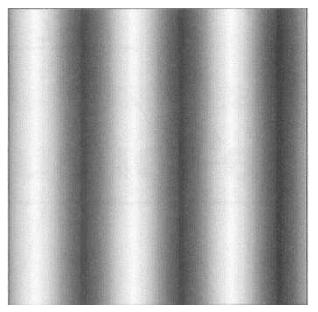
\includegraphics[width=0.5\linewidth]{img/Screenshot 2025-10-01 132803.png}
    \caption{Ảnh $f(x,y)$}
\end{figure}

\end{enumerate}
\section{Khác biệt giữa miền không gian và miền tần số}
Trong miền không gian, ta xử lý trực tiếp trên từng điểm ảnh, còn trong miền tần số ta xử lý dựa trên tốc độ thay đổi giá trị của điểm ảnh trên miền không gian.

\begin{enumerate}
    \item Miền không gian: Ma trận ảnh đầu vào $\rightarrow$ Xử lý $\rightarrow$ Ma trận ảnh đầu ra.

    \item Miền tần số: Ảnh vào $\rightarrow$ Phân bố tần số $\rightarrow$ Xử lý $\rightarrow$ Chuyển đổi ngược $\rightarrow$ Ảnh ra.

    Miền tần số không gian có thể tạo ra mối quan hệ chu kỳ rỡ ràng trong miền không gian, trong miền tần số, một số toán tử xử lý ảnh sẽ trở nên hiệu quả hơn.

    Trong nhiều trường hợp, người ta dùng chuyển đổi Fourier để chuyển ảnh từ miền không gian sang miền tần số.
\end{enumerate}
\section{Khái niệm chuỗi Fourier và biến đổi Fourier}

     Chuỗi Fourier (Fourier series) được nhà Toán học người Pháp tên Jean Baptiste Joseph Fourier đưa ra vào thế kỷ 19. Ông khẳng định rằng với bất kỳ hàm số $f(t)$ tuần hoàn với chu kỳ $T$ đều có thể biểu diễn được dưới dạng tổng của các hàm số sine và cosine với những tần số khác nhau, mỗi hàm số nhân với một hệ số tương ứng. Khi đó, ta gọi tổng các chuỗi hàm số sine và cosine này là chuỗi Fourier.

		 Giống như chuỗi Taylor, chuỗi Fourier là một dạng đặc biệt của khai triển hàm số. 
		 Với chuỗi Taylor, ta quan tâm đến tập các hàm số đặc biệt dạng như sau: 
		\begin{equation}
		\tag{a}
		1,x,x^2,x^3,\ldots
		\end{equation}
		 còn với chuỗi Fourier, ta quan tâm đến các dạng hàm đặc biệt lượng giác:
		\begin{equation}
		\tag{b}
		1,\cos x, \cos 2x, \cos 3x,\ldots,\sin x,\sin 2x,\sin 3x,\ldots
		\end{equation}
		Do đó, khai triển chuỗi Fourier của một hàm số $f$ sẽ có dạng tổng các hàm lượng giác $\sin$ và $\cos$ cùng các hệ số:
		\begin{equation}
			\tag{c}
			f(x) = a_0 + \sum_{n=1}^{+\infty}a_n\cos nx + b_n\sin nx,
		\end{equation}
với 
\[a_0 = \dfrac{1}{2\pi}\int\limits_{-\pi}^{\pi}f(x)dx,\]
\[a_n = \dfrac{1}{\pi}\int\limits_{-\pi}^{\pi}f(x)\cos nxdx,\quad n=1,2,\ldots\]
\[b_n = \dfrac{1}{\pi}\int\limits_{-\pi}^{\pi}f(x)\sin nxdx,\quad n=1,2,\ldots\]

     \begin{figure}[H]
		 \centering
		 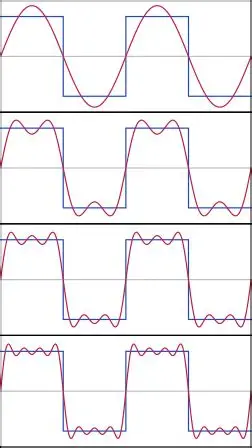
\includegraphics[width=5cm]{img/fourier.png}
		 \caption{Minh họa về chuỗi Fourier và các dạng hàm sóng tương ứng từ trên xuống với chỉ số $n$ càng lớn.}
		 \end{figure}
		 \begin{figure}[H]
		 \centering
		 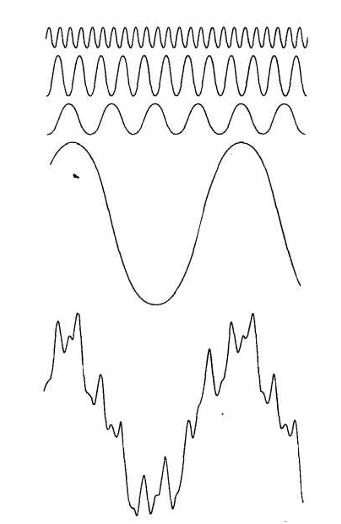
\includegraphics[width=5cm]{img/fourier1.png}
		 \caption{Minh họa chuỗi Fourier}
		 \end{figure}
\subsection{Biến đổi Fourier cho hàm liên tục}
\subsubsection{Biến đổi Fourier cho hàm một biến số}
Lấy $f$ là hàm trơn từng khúc tuần hoàn chu kì $T$. Dạng phức của chuỗi Fourier của $f$ là: 
\begin{dl}	
\textbf{\textit{(Dạng phức của chuỗi Fourier)}}
\begin{equation}
	\label{131}
    f(t)= \sum_{n=-\infty} ^{\infty} c_ne^{i\dfrac{2\pi n}{T}t},
\end{equation}
với hệ số Fourier $c_n$ được cho bởi
\begin{equation}
	\label{132}
    c_n=\dfrac{1}{T}\displaystyle\int\limits_{-\frac{T}{2}}^{\frac{T}{2}} f(t)e^{-i\dfrac{2\pi n}{T}t}dt,\quad n=0,\pm 1,\pm 2, \pm 3,...
\end{equation}
\end{dl}
Phương trình (\ref{131}) là cách khai triển hàm số $\sin$ và $\cos$ theo công thức Euler trong trường số phức:
\begin{equation}
	\label{133}
    e^{i\varphi}=\cos\varphi+i \sin\varphi
\end{equation}
Đối với những hàm số không có tính tuần hoàn, nhưng diện tích dưới đường cong của hàm số đó là hữu hạn, ta có thể biểu diễn hàm số đó dưới dạng tích phân của hàm $\sin$ và $\cos$ nhân với hàm trọng số. Biểu thức thu được gọi là biến đổi Fourier.
Ta xác định phương trình biến đổi Fourier của một hàm số liên tục $f(t)$ có biến t liên tục như sau:
\begin{equation}
	\label{134}
    \mathcal{F}\{f(t)\}(\mu)=\int\limits_{-\infty}^{+\infty}f(t)e^{-2\pi i  \mu t}dt
\end{equation}
với $\mu$ là biến liên tục. Vì khi lấy xong tích phân sẽ mất t nên ta chỉ còn lại $\mu$, vậy ta sẽ ký hiệu lại phương trình biến đổi Fourier cho rõ ràng hơn như sau:

\begin{equation}
	\label{135}
  \hat{f}(\mu)=\int\limits_{-\infty}^{+\infty}f(t)e^{-2\pi i \mu t}dt
\end{equation}

Ngược lại, cho trước $\hat{f}(\mu)$, ta có thể tìm lại $f(t)$ bằng cách sử dụng chuyển đổi ngược Fourier (inverse Fourier transform), $f(t)=\mathcal{F}^{-1}\{\hat{f}(\mu)\}$, viết là:

\begin{equation}
	\label{136}
    f(t)=\int\limits_{-\infty}^{+\infty}\hat{f}(\mu)e^{2\pi i \mu t}d\mu,
\end{equation}

sử dụng công thức Euler, ta viết lại phương trình (\ref{135}) như sau:

\begin{equation}
	\label{137}
     \hat{f}(\mu)=\int\limits_{-\infty}^{+\infty}f(t)[\cos(2\pi\mu t)-i\sin(2\pi\mu t)]dt.
\end{equation}

Biến còn lại khi lấy tích phân là $\mu$, chính là tần số của hàm lượng giác nên miền của chuyển đổi Fourier là miền tần số.

\subsubsection{Biến đổi Fourier cho hàm hai biến số}

Ta có công thức biến đổi Fourier và biến đổi Fourier ngược cho hàm hai biến như sau:

Biến đổi Fourier thuận:
\begin{equation}
\mathcal{F}(u,v) = \int\limits_{-\infty}^{+\infty}\int\limits_{-\infty}^{+\infty}f(x,y)e^{-2\pi i(ux+vy)}dxdy
\end{equation}

Biến đổi Fourier ngược:
\begin{equation}
\mathcal{F}^{-1}(u,v) =f(x,y)= \int\limits_{-\infty}^{+\infty}\int\limits_{-\infty}^{+\infty}f(x,y)e^{2\pi i(ux+vy)}dudv
\end{equation}



\subsection{Biến đổi Fourier cho hàm rời rạc}

Vì các điểm ảnh là các điểm dữ liệu rời rạc nên ta áp dụng biến đổi Fourier, ta cần xây dựng một công thức sử dụng cho các biến rời rạc.

\subsubsection{Hàm một biến số}

Giả sử ra có bộ dữ liệu dãy $x_n$, (với $n= 1,2,3,...,N)$, ta xác định DFT(Discrete Fourier Transforms) cho $x_n$ như sau: 
\begin{equation}
	\label{144}
    \mathcal{X}_n= \dfrac{1}{N}\sum_{i=1}^Nx_ke^{\dfrac{-ik2\pi n}{N}},\quad n=\overline{1,N}.
\end{equation}
Biến đổi Fourier ngược(IDFT) là
\begin{equation}
	\label{145}
    x_n =\sum_{k=1}^N\mathcal{X}_ne^{\dfrac{ik2\pi n}{N}},\quad n=\overline{1,N}.
\end{equation}
Về bản chất, biến đổi Fourier có sử dụng số phức. Nhưng trong xử lý ảnh ta quan tâm đến phần số thực để làm, do đó xem phần ảo bằng $0$.
\subsubsection{Hàm hai biến số}
Giả sử hàm $f(x,y)$ là ảnh đầu vào, DFT cho hàm hai biến này là: 
\begin{equation}
\mathcal{F}(u,v) = \dfrac{1}{MN}\sum_{x=1}^{M}\sum_{y=1}^{N} f(x,y)e^{-2\pi i\left(\frac{ux}{M}+\frac{vy}{N}\right)}
\end{equation}
\begin{equation}
\mathcal{F}^{-1}(u,v)=f(x,y) =\sum_{u=1}^{M}\sum_{v=1}^{N} \mathcal{F}(u,v)e^{2\pi i\left(\frac{ux}{M}+\frac{vy}{N}\right)}
\end{equation}
\subsection{Biến đổi Fourier nhanh(FFT)}
\subsubsection{Hàm một biến số}
Để chuyển ảnh từ miền không gian sang miền tần số bằng cách sử dụng chuyển đổi Fourier thông thường đòi hỏi chi phí lớn $(O(N^2)$ với $N$ là số điểm ảnh).

Thuật toán FFT thông dụng nhất là thuật toán do J.W.Cooley và John Tukey đề xuất, tính chuyển đổi Fourier cho các giá trị rời rạc bằng cách sử dụng đệ quy tính các giá trị ở vị trí chẵn lẻ. 


\begin{equation}
	\label{1314}
\mathcal{X}_k = \underbrace{\sum_{m=1}^{\dfrac{N}{2}}x_{2m}e^{-\dfrac{2\pi i}{N}(2m)k}}_{ \text{DFT cho phần chẵn}} + \underbrace{\sum_{m=1}^{\dfrac{N}{2}}x_{2m+1}e^{-\dfrac{2\pi i}{N}(2m+1)k}}_{\text{DFT cho phần lẻ}}.
\end{equation}
\begin{equation}
	\label{1315}
\mathcal{X}_k = \sum_{m=1}^{\dfrac{N}{2}}x_{2m}e^{-\dfrac{2\pi i}{N/2}mk} + e^{-\dfrac{2\pi i }{N}k}\sum_{m=1}^{\dfrac{N}{2}}x_{2m+1}e^{-\dfrac{2\pi i}{N/2}mk}.
\end{equation}

Ta có thể viết lại $X_k$ cho gọn hơn như sau: 
\begin{equation}
	\label{1316}
\mathcal{X}_k = E_k + e^{-\dfrac{2\pi i }{N}k}O_k,
\end{equation}
với $E_k, O_k$ lần lượt là tổng các phần chẵn và phần lẻ.

Do tính tuần hoàn có chu kỳ của DFT nên
\begin{equation}
    E_{k+\tfrac{N}{2}} = E_k
\end{equation}
và
\begin{equation}
    O_{k+\tfrac{N}{2}} = O_k
\end{equation}

Khi đó, ta viết lại phương trình (\ref{1314}) và (\ref{1315}) thành
\begin{equation}
	\label{1319}
    \mathcal{X}_k = 
    \begin{cases}
        E_k + e^{-\tfrac{2\pi i}{N}k} O_k, & 0 \leq k < \tfrac{N}{2} \\
        E_{k-N/2} + e^{-\tfrac{2\pi i}{N}k} O_{k-N/2}, & \tfrac{N}{2} \leq k < N
    \end{cases}
\end{equation}

Mặt khác, $e^{-\tfrac{2\pi i}{N}k}$ hình thành từ:
\begin{equation*}
    e^{-\tfrac{2\pi i}{N}(k+N/2)} 
    = e^{-\tfrac{2\pi i}{N}k - \pi i} 
    = e^{-\pi i} e^{-\tfrac{2\pi i}{N}k} 
    = -e^{-\tfrac{2\pi i}{N}k}
\end{equation*}

Khi đó, ta có thể giảm khối lượng tính toán xuống một nửa. Với $0 \leq k < N/2$, từ phương trình (\ref{1319}) ta được:
\begin{equation}
    \mathcal{X}_k = E_k + e^{-\tfrac{2\pi i}{N}k} O_k
\end{equation}
\begin{equation}
    \mathcal{X}_{k+N/2} = E_k - e^{-\tfrac{2\pi i}{N}k} O_k
\end{equation}


\begin{lstlisting}[caption={Thuật toán FFT đệ quy dạng ditfft2}, label={code:fft}]
import cmath

def ditfft2(x, N, s):
    """
    x: list day so (co the la phuc)
    N: kich thuoc FFT (phai la luy thua cua 2)
    s: buoc nhay (stride)
    """
    if N == 1:
        return [x[0]]  # Truong hop co so
    
    # Tinh FFT phan chan va le
    X_even = ditfft2(x[0::2*s], N//2, 2*s)  # (x0, x2s, x4s, ...)
    X_odd  = ditfft2(x[s::2*s], N//2, 2*s)  # (xs, x3s, x5s, ...)
    
    X = [0] * N
    for k in range(N//2):
        t = X_even[k]
        exp_term = cmath.exp(-2j * cmath.pi * k / N) * X_odd[k]
        X[k] = t + exp_term
        X[k + N//2] = t - exp_term
    
    return X
\end{lstlisting}
\subsubsection{Hàm hai biến số}
Từ ý tưởng của hàm một biến, ta có thể tính được FFT của hàm hai biến bằng cách tính theo một chiều với mỗi giá trị của biến $x$(theo từng cột). Sau đó tính ngược lại theo $y$(theo từng hàng) với giá trị thu được ở trên.

Trong Python, ta có thể sử dụng hàm \texttt{fft2} để đưa ảnh sang chuỗi Fourier và dùng \texttt{ifft2} để trả ngược lại ảnh lúc đầu.
\subsection{Định lý tích chập}
Trong xử lý ảnh hoặc tăng cường ảnh trong miền không gian, người ta sử dụng khái niệm về tích chập , trong đó ảnh sau khi được xử lý bằng tích chập của ảnh ban đầu và bộ lọc ảnh tạo thành. Về mặt Toán học, ta giả sử hai hàm số liên tục, ta có định nghĩa tích chập $*$ của hai hàm số này như bên dưới.

\begin{equation}
	\label{1322}
f(t) \ast g(t) = \int\limits_{-\infty}^{+\infty}f(\tau)g(t -\tau)d\tau.
\end{equation}
Ta áp dụng tích chập cho hàm hai biến sau khi biến đổi Fourier như sau: 
\begin{equation}
\label{1323}
\mathcal{F}\{f(t)\ast g(t)\} = \int\limits_{-\infty}^{+\infty}\left[\int\limits_{-\infty}^{+\infty}f(\tau)g(t-\tau)d\tau\right]e^{-2\pi i\mu t}dt,
\end{equation}
từ đây ta có: 
\begin{align*}
\mathcal{F}\{f(t)\ast g(t)\} &= \int\limits_{-\infty}^{+\infty}f(\tau)\left[\int\limits_{-\infty}^{+\infty}g(t-\tau)e^{-2\pi i\mu t}d\tau\right]dt\\
&=\int\limits_{-\infty}^{+\infty}f(\tau)e^{-2\pi i \mu t}d\tau\int\limits_{-\infty}^{+\infty}g(u)e^{-2\pi i\mu u}du\\
&=\mathcal{F}(f)(\mu)\mathcal{F}(g)(\mu)=\hat{f}(\mu)\hat{g}(\mu).
\end{align*}
Vậy giả sử $\mathcal{F}\{f(t)\} = \hat{f}(\mu), \mathcal{F}\{g(t)\} = \hat{g}(\mu)$, khi đó: 
\begin{equation}
\mathcal{F}\{f(t)\ast g(t)\} = \hat{f}(\mu)\hat{g}(\mu).
\end{equation}
Áp dụng cho trường hợp hai chiều, giả sử $f(x,y)$ là ảnh đầu vào, $h(x,y)$ là bộ lọc ảnh, $\mathcal{F}\{f(x,y)\}=\hat{f}(\mu,\eta)$, $\mathcal{F}\{g(x,y)\} = \hat{g}(\mu,\eta)$, khi đó
\begin{equation}
\mathcal{F}\{f(x,y)\ast g(x,y)\} = \hat{f}(\mu,\eta)\hat{g}(\mu,\eta).
\end{equation}

\section{Xử lý ảnh trong miền tần số}
\subsection{Khái niệm về xử lý ảnh trong miền tần số}
Khi chụp ảnh, ta có thể thu được các ảnh có tần số thấp (sự thay đổi mức xám của ảnh ít, ví dụ như ảnh một bức tường) hay ảnh có tần số cao (ví dụ như biên của vật thể). Vì vậy, ta cần có bộ lọc $H(u,v)$ có thể làm giảm đi tần số cao trong khi đi qua các tần số thấp (gọi là lọc thông thấp) làm cho ảnh mờ đi. Ngược lại, ta cần có bộ lọc có tính chất ngược với lọc thông thấp (gọi là lọc thông cao) giúp tăng cường chi tiết hình dạng vật thể, đồng thời làm giảm độ tương phản ảnh. Hình ảnh sau mô tả điều này.



Định lý tích chập cho ta mối quan hệ giữa miền không gian và miền tần số, cụ thể, thông qua tích chập, một ảnh trong miền không gian có thể chuyển qua miền tần số và ngược lại.

Quy trình lọc ảnh trong miền tần số như sau:
\[\text{Ảnh}\rightarrow\text{Biến đổi Fourier}\rightarrow\text{Lọc}\rightarrow\text{Biến đổi Fourier ngược}
\rightarrow\text{Ảnh}\]
\begin{enumerate}
\item Bước 1: Xử lý ảnh trong miền không gian, tức tăng hoặc giảm độ sáng của ảnh.
\item Bước 2: Lấy DFT của ảnh.
\item Bước 3: Canh giữa DFT, tức mang DFT từ góc ảnh ra giữa ảnh, trong Matlab ta sử dụng hàm shififft để thực hiện.
\item Bước 4: Thực hiện tích chập với hàm lọc.
\item Bước 5: Trượt DFT từ giữa ảnh ra góc.
\item Bước 6: Lấy chuyển đổi ngược IDFT, tức chuyển ảnh từ miền tần số sang miền không gian.
\end{enumerate}
\subsection{Các bộ lọc băng thông trong miền tần số}

Khái niệm bộ lọc trong miền tần số tương tự như khái niệm mặt nạ trong miền không gian.

Sau khi chuyển ảnh sang miền không gian, ta áp dụng một số bộ lọc trong quy trình lọc ảnh nhằm làm mờ ảnh, giảm nhiễu ảnh hoặc làm rõ-làm nét ảnh.

Các bộ lọc thông dụng:
\begin{enumerate}
\item Lọc thông thấp/cao Ideal (Ideal low/high pass filter)
\item Lọc thông thấp/cao Gaus (Gaussian low/high pass filter
).

\item Lọc thông thấp/cao Butterworth (Butterworth low/high pass filter).



\end{enumerate}

Ta sẽ đi qua một số ứng dụng của bộ lọc này.

\section{Tổng kết chương}

	\chapter*{Kết luận}                         % Chương 3
	\addcontentsline{toc}{chapter}{{\bf  Kết luận}\rm}
	\indent
	\thispagestyle{fancy}
	

Bài báo cáo này đạt được các vấn đề sau đây:
	
	\begin{itemize}
	\item Chương 1:
	

	
	\item Chương 2:

	
	\item Chương 3: 
	

	
	\end{itemize}
	
	\begin{thebibliography}{99}
		\addcontentsline{toc}{chapter}{{\bf  Tài liệu tham khảo}} 
		\thispagestyle{fancy}
		%	\item[\textbf{\large 1.}] \textbf{\large Tài liệu tham khảo chính thức}
		
		%\item[\textbf{\large 1.}] \textbf{\large Tài liệu tham khảo chính thức}
		
		
		%Các tài liệu chính được tôi chọn lựa để tham khảo khi thực hiện luận văn là  tài liệu số \cite{Mat}, \cite{Gab1} và \cite{Gian}. 	Các vấn đề liên quan được chúng tôi khảo cứu trong các tài liệu còn lại.
		

		
		\bibitem{M} Michael Bartholomew-Biggs - Nonlinear Optimization with Engineering Applications (2008, Springer).
		
	%	\bibitem{H} Hu T.C.-Linear and Integer Programming Made Easy.
		
	%	\bibitem{L} Linear Programming - Foundations and Extensions - Springer US (2001).
		
	%	\bibitem{BB} Bùi Phúc Trung, Nguyễn Thị Ngọc Thanh, Vũ Thị Bích Liên,\textit{ Giáo trình Quy hoạch tuyến tính Tối ưu hóa}, NXB Lao Động-Xã Hội-2003.
		
	%	\bibitem{H} H. A. Eiselt · C.-L. Sandblom-Linear Programming
	%	and its Applications.
	%	\bibitem{P} Phan Hoàng Chơn,\textit{ Giáo trình Đại Số Tuyến tính}, Đại học Sài Gòn, 2023. 
		
	%	\bibitem{Đ} Nguyễn Hữu Điển, \textit{Giáo trình tối ưu tuyến tính và ứng dụng }, NXB Đại học Quốc gia Hà Nội, 2018. 
	%	\bibitem{B} Bùi Minh Trí, \textit{Tối ưu hóa tập I}, Trường Đại học Bách Khoa Hà Nội,NXB Khoa học và Kỹ thuật.
		
	%			\bibitem{T}   Tạ Quang Sơn, \textit{Bài giảng Quy hoạch tuyến tính}, Đại học Sài Gòn, 2023.
		
	%	\bibitem{TT}   Tạ Quang Sơn, \textit{Bài giảng Quy hoạch phân thức tuyến tính}, Đại học Sài Gòn, 2022.
		
	\end{thebibliography}
	
	\newpage % Add a new page after the bibliography
	
	\thispagestyle{empty} % Ensure the new page is completely blank

	\mbox{}

\end{document}